\subsection{Notation}
\TODO{Notation needs to be introduced in the background section, Tiling should be the first subsection}
We represent a decision tree by $\Tree = (V, E, r)$ where $V$ is the set of nodes, $E$ the set of edges and
$r \in V$ is the root. For each node $n \in V$, we define the following.
\begin{enumerate}
    \item $threshold(n) \in \mathbb{R}$, the threshold value for $n$.
    \item $featureIndex(n) \in \mathbb{N}$, the feature index for $n$.
    \item $left(n) \in V$, the left child of $n$ or $\emptyset$ if $n$ is a leaf. If $left(n) \neq \emptyset$, then $(n, left(n)) \in E$.
    \item $right(n) \in V$, the right child of $n$ or $\emptyset$ if $n$ is a leaf. If $right(n) \neq \emptyset$, then $(n, right(n)) \in E$.
\end{enumerate}
We use $L_{\Tree} \subseteq V$ to denote the set of leaves. % subseteq because tree could have single node

\subsection{Tiling}
\label{sec:Tiling}
% Treebeard vectorizes tree walks by grouping nodes of a decision tree into \textbf{\emph{tiles}}. The nodes in a tile are evaluated concurrently using vector instructions. Once the nodes of the current tile are evaluated, a look up table is used to compute which child of the current tile to move to next.

While a decision tree is naturally represented by a binary tree, 
it is not the best representation for tree traversal as it (i) requires many memory accesses, 
(ii) has poor branching structure and (iii) cannot make use of vector instructions. 
This section proposes a tiling optimization where we group multiple nodes in a decision tree into a single tile, effectively transforming a binary tree into an $n$-ary tiled tree. This not only allows the compiler to generate vectorized code (see Section~\ref{sec:Vectorization} ) to traverse trees but also enables spatial locality improvements by grouping nodes that are likely to be accessed together. We demonstrate this with two tiling heuristics later in the section. 



\CommentOut{
Treebeard groups nodes of the decision tree into \textbf{\emph{tiles}}. Tiling provides two benefits. 
\begin{enumerate}
  \item It allows the compiler to generate vector code to traverse trees. Section \ref{sec:Vectorization} describes how Treebeard does this.
  \item It enables spatial locality improvements by grouping together nodes that are likely to be accessed together. 
\end{enumerate}
Once nodes are grouped into tiles, an $n$-ary tree whose nodes are tiles is constructed. Treebeard then generates 
optimized code to walk this tree. The listing below shows at a high level how a tiled tree is walked (This is not 
true IR, but presented for clarity). 
}

Once trees are tiled Treebeard generates tree walks with the code structure shown below.
\begin{lstlisting}[style=c++]
  ResultType Prediction_Function(...) {
    // ...
    Tile t = getRootTile(tree)
    while (!isLeaf(tree, t)) do {
      // Evaluate predicates of all nodes in the tile
      predicates = evaluateTilePredicates(t, rows[i])
      
      // Move to the correct child of the current tile
      t = getChildTile(tree, t, predicates) 
    }
    treePrediction = getLeafValue(t)
    // ...
  }  
\end{lstlisting}
The code is just an abstract representation of a tiled tree walk that enables efficient lowering of specific steps in subsequent stages. 
\op{evaluateTilePredicates} (speculatively) computes the predicates on all nodes in a tile (line 6). Then \op{getChildTile} (line 9), uses the computed predicate values to determine which child of the current tile to move to. We defer a description of how these operators are lowered to a later section but focus on tiling algorithms in this section.

\CommentOut{
To compute the prediction of the tree, the predicates of all nodes in the tile are computed simultaneously (line 6). 
Then, the computed predicate values are used to determine which child of the current tile to move to (in the 
$n$-ary tree). This section presents the details of tiling and how Treebeard's general tiling infrastructure 
can be used to develop tiling algorithms with different objectives (sections \ref{sec:UnifTiling}) and \ref{sec:ProbTiling}).
The details of how Treebeard lowers predicate evaluation and moving to the correct child to use vector instructions 
are described in section \ref{sec:Vectorization}.

\subsection{Tiles and Tree Tiling}
\label{sec:ValidTiling}
}
\subsection*{Conditions for Efficient Tiling}
\label{sec:ValidTiling}
While any arbitrary partitioning of the nodes of a tree could be considered for tiling we impose a few intuitive constraints.
% to only allow nodes that are likely to be accessed together to be grouped into a tile. 
\TODO{kr : replace $n_t$ with sz?}
Given a tree $\Tree = (V, E, r)$ and a tile size $n_t$ we impose the following constraints on the generated tiles $\{ T_1, T_2, ... ,T_m \}$ .
\begin{description}
    \item[Partitioning] $T_1 \cup T_2 ... \cup T_m = V$ and $T_i \cap T_j = \emptyset$ for all $i\neq j$
    \item[Connectedness] If $u, v \in T_i$, there is a (undirected) path connecting $u$ and $v$ fully contained in $T_i$.
   \item [Leaf seperation] $\forall l \in L_{\Tree}$ : $l \in T_i \rightarrow v \notin T_i \;\; \forall v \in V \backslash \{l\}$
  \item [Maximal tiling] if there are tiles such that. $|T_i| < n_t$ then there is no $v \in V\backslash \{ T_i \cup L_{\Tree} \}$ such that $(u, v) \in E$ for some $u \in T_i$. 
\end{description}
The \textbf{partitioning} and \textbf{maximal tiling} constraints together ensure that we group nodes into as few tiles as possible. {\textbf{Connectedness}} ensures that each tile is a sub-tree, a natural grouping of nodes that are likely to be accessed together. The {\textbf{Leaf separation}} constraint ensures that leafs are not tiled along with internal nodes. Leafs in a decision tree need special handling, they are used to check for walk termination and to determine the output (prediction). This constraint ensures that tiles are homogenous, this in-turn allows us to specialize the in-memory layout of trees and also simplifies code generation. We discuss leaf handling and tree layout in Section~\ref{sec:}.
We refer to any tiling that satisties the above constraints as a \emph{valid} tilling.

%%% COMMENT %%%% 
\CommentOut{
\subsection{Tiled Trees}
A tiling transformation communicates the tiling to the Treebeard infrastructure by assigning a tile ID to each node in the decision tree. Using these tile IDs, Treebeard checks the validity of the tiling and then contructs a tree whose nodes are tiles. We call this tree the \textbf{\emph{tree of tiles}}. \TODO{We need a better name for this}
Figure \ref{Fig:ValidTilingTileSize3} shows a valid tiling with tile size 3 and the tree of tiles constructed by Treebeard. Three nodes are grouped into each of the tiles $t_1$ and $t_2$ as shown. Each tile is collapsed into a single node in the tree of tiles. However, each leaf in the original tree becomes a leaf in the tree of tiles.

\begin{figure}
  \centering
  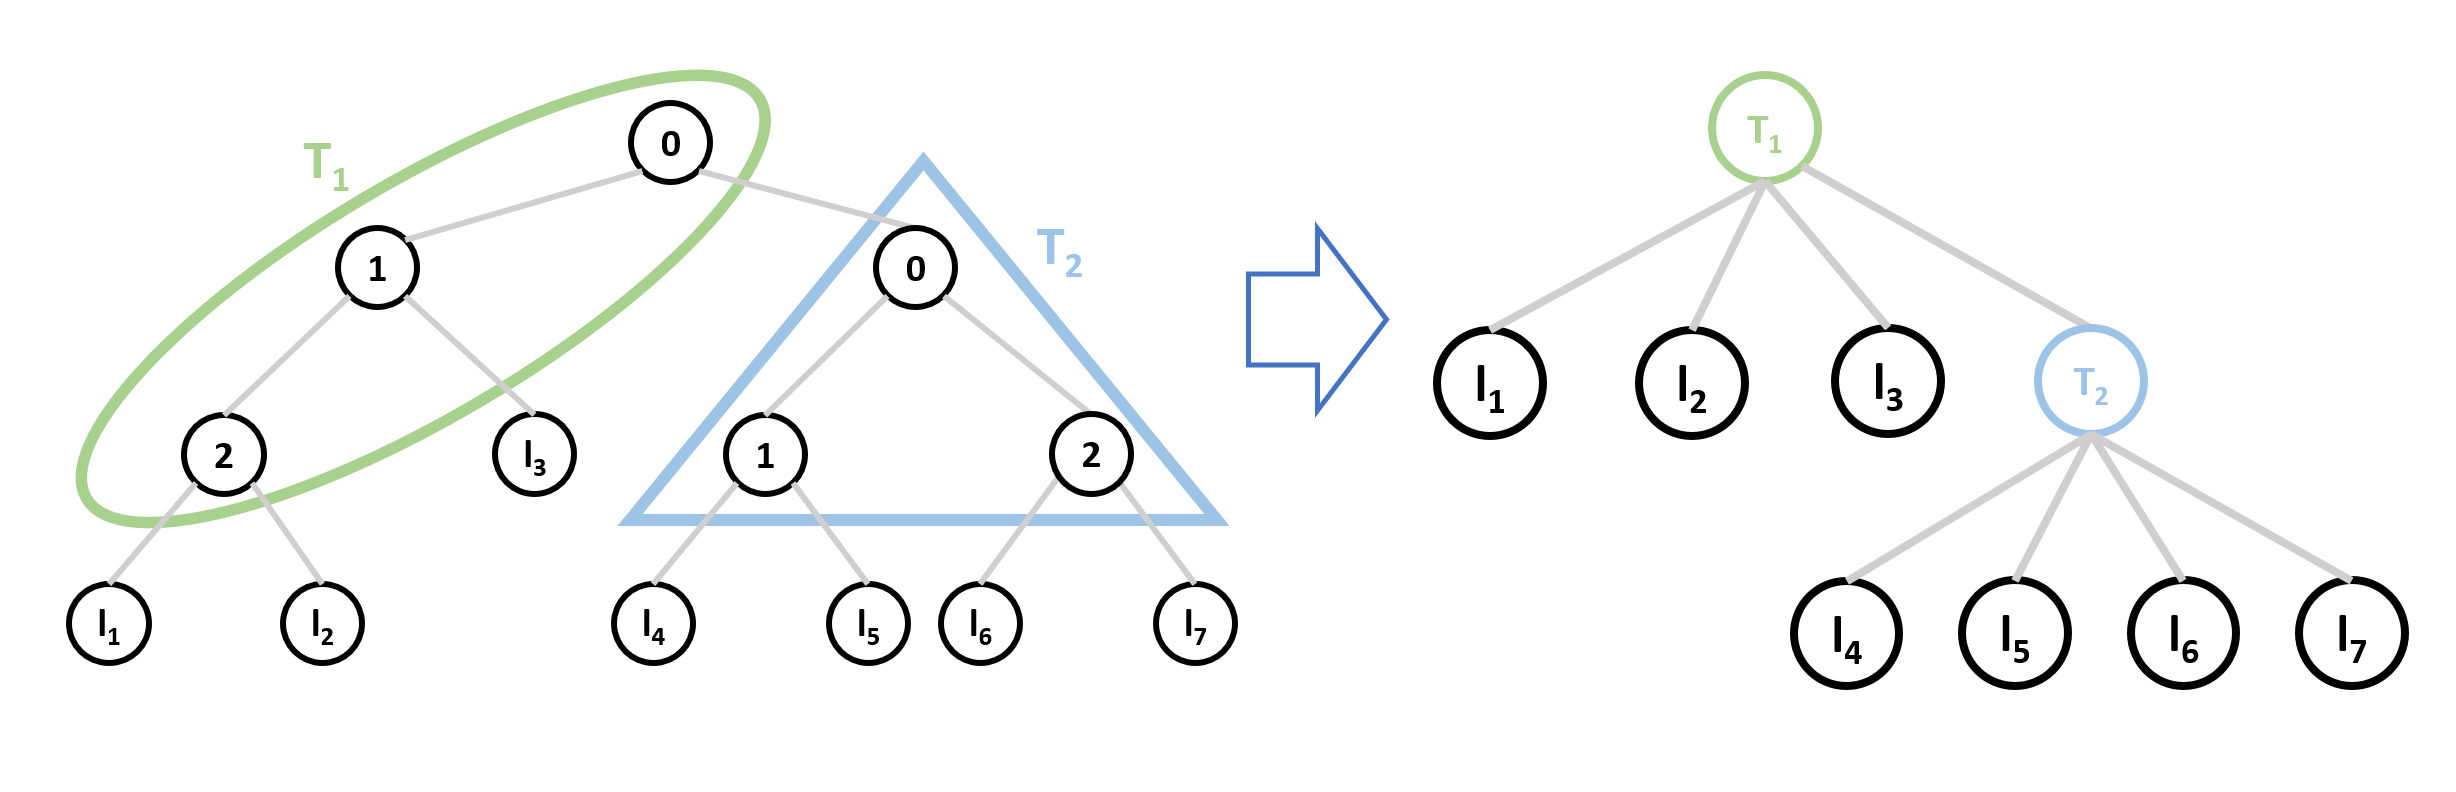
\includegraphics[width=\linewidth]{figures/TiledTree_Size3.PNG}
  \caption{Example of a valid tree tiling with tile size $n_t=3$}
  \label{Fig:ValidTilingTileSize3}
\end{figure}

Treebeard maintains the following invariants.
\begin{enumerate}
  \item All tiles in a tree are the same size $n_t$. If the tiling produces any smaller tiles, these are padded by inserting dummy nodes to make them the required size.
  \item Nodes within tiles are always ordered in level order and left to right within a level. The numbering of the nodes in the above diagram shows this node order.
  \item Children of a node are numbered from left to right (regardless of level). For example, $l_1$ is the first child of $t_1$, $l_2$ is the second and so on.
\end{enumerate}
}
%%% END COMMENT %%%%

\subsection{Basic Tiling Algorithm}
\label{sec:UnifTiling}
% The justification for uniform tiling -- if we assume all paths are equally likely,
% we want to minimize the depth of speculation
Algorithm~\ref{Alg:UnifTilingAlgo} shows a simple tiling algorithm that satisfies all the above constraints. 
Tiling starts at the root and constructs a tile $Tile$ by performing
a level order traversal. The call \op{LevelOrderTraversal(r, $n_t$)} picks the next $n_t$ nodes according to the standard level order tree traversal algorithm (not described here) applied only to internal nodes of the tree. Once the current tile is constructed, the tiling procedure is recursively performed on all nodes that are 
destinations for edges going out of the constructed tile.
It is easy to see that the set of tiles constructed by algorithm \ref{Alg:UnifTilingAlgo} satisfies the constraints above.
\TODO{Pass a modified tree without leafs to the level order traversal call. Explicitly add leaves as seperate tiles}
% Algorithm for uniform tiling
\begin{algorithm}
  \caption{Uniform tree tiling}
  \label{Alg:UnifTilingAlgo}
  \begin{algorithmic}
      \Procedure{TileTree}{$tree = (V, E, r)$, $n_t$} 
          \If {$r \in L$}
              \State \textbf{return} $\{ r \}$
          \EndIf
          \State \textcolor{codegreen}{\textit{//Level order traversal to collect $n_t$ or fewer nodes. }}
          \State \textcolor{codegreen}{\textit{//Leaves are not included in the constructed tile. }}
          \State $Tile \leftarrow LevelOrderTraveral(r, n_t)$
          \State $Tiles =  \{ Tile \}$
          \For{$(u,v) \in Out(Tile)$}
              \State $Tiles \leftarrow Tiles \cup TileTree(S_v, n_t)$
          \EndFor
          \State \textbf{return} $Tiles$
      \EndProcedure
  \end{algorithmic}
\end{algorithm}

One interesting property of this tilling algorithm is that it naturally reduces the imbalance in trees, especially at large tile sizes. As the algorithm traverses down to sparser level of the tree, it naturally groups sub-trees containing chains of nodes, thus balancing the trees. While its possible to further enhance the algorithm to explicitly balance tiled trees, we find that basic tiling suffices in practice.
\CommentOut{
\subsubsection{Further Opimization and Code Generation}
We found that most leaf tiles for a given tree are at the same depth when uniform tiling is used. Furthermore, we see that deeper leaves 
are more likely to be reached.
%\footnote{Intuitively, this is true because training algorithms keep splitting nodes to maximize gain and gain
%will typically be maximized by splitting a large number of inputs.}.
Based on these observations, we (optionally) pad the tree of tiles generated with uniform tiling so that all leaves are at the same depth.
This transformation is performed on the high level IR after uniform tiling. 
Once the trees have been padded to make all leaves equal depth, the tree walks are fully unrolled to evaluate a fixed 
number of tiles and all leaf checks are omitted.

One other complication the code generator needs to handle is the fact that different trees in the model being 
compiled potentially have different depths. In order to handle
this, Treebeard sorts the trees by their depth. This ensures that all trees with equal depth are grouped together. Once this is done, 
the loop over the trees is fissed so that each of the resulting loops only walks trees of a single depth. Consider for example a 
forest with 4 trees $T_1$, $T_2$, $T_3$, and $T_4$ in that order. Further, assume that $T_1$ and $T_4$ have depth 2 while $T_2$ and $T_3$
have depth 3. First, Treebeard reorders the trees to be in the order $T_1$, $T_4$, $T_2$, $T_3$. Then, the loop over the trees is fissed
as shown in the following listing.

% loop transformations for uniform tiling (splitting) 
\begin{lstlisting}{style=c++}
  forest = ensemble(...)
  for i = 0 to batchSize step 1 {
    prediction = 0
    for t = 0 to 2 step 1 {
      tree = getTree(forest, t) 
      node = getRoot(tree)
      node = traverseTreeTile(tree, node, rows[i])
      treePrediction = getLeafValue(tree, node)
      prediction = prediction + treePrediction
    }
    for t = 2 to 4 step 1 {
      tree = getTree(forest, t) 
      node = getRoot(tree)
      node = traverseTreeTile(tree, node, rows[i])
      node = traverseTreeTile(tree, node, rows[i])
      treePrediction = getLeafValue(tree, node)
      prediction = prediction + treePrediction
    }
    predictions[i] = prediction
  }  
\end{lstlisting}

\TODO{AP: This listing is unnecesarily long. Can we maybe leave out the loop bodies and say something like "depth 2 walk"? Should 
we point to the figure in the overview section instead?}
}
\subsection{Probability Based Tiling}
\label{sec:ProbTiling}
%\subsubsection*{Motivation}

The next algorithm we propose exploits the inherent biases among the leaves of a decision tree. In typical machine learning models some leafs (equivalently outcomes or predictions) are more likely to be reached than others. In such settings, having balanced tiled trees is not sufficient to minimize expected inference time. 

Consider for example two machine learning models \op{airline-ohe} and \op{epsilon} (also used in our evaluation). 
Consider the graphs shown in   
figures \ref{Fig:AirlineOHEStats} and \ref{Fig:EpsilonStats} that are generated from training data. Each line in these graphs corresponds to a fixed fraction of the input (say $f$). 
A point on a line at coordinate $(x, y)$ means that a fraction $y$ of trees in the model could cover a fraction $f$ of all training inputs with a fraction $x$ of 
leaves. For example, the first point on the $f=0.9$ line in figure \ref{Fig:AirlineOHEStats} says that about 52\% of trees ($y$ value) need only 1\% of their
leaves ($x$ value) to cover 90\% of the training input. 
In general, Figure \ref{Fig:AirlineOHEStats} shows that very few leaves are needed to cover a very large fraction of inputs for the benchmark \op{airline-ohe}. 
This means that a small fraction of leaves are very likely. 
We call trees with a small number of extremely likely leaves \textbf{\emph{leaf biased}}.

On the other hand, for the benchmark \op{epsilon},
figure \ref{Fig:EpsilonStats} shows that a trees need a much larger fraction of their leaves to cover a significant fraction of the training input.
This means that most trees in \op{epsilon} are not leaf biased.

\CommentOut{
\subsubsection{More Notation}
In order to formulate the probability based tiling algorithm as an optimization problem, we define the following.
\begin{enumerate}
    \item For every leaf $l \in L$, we define $p_l$ as the probability that the leaf $l$ is reached.
    \item For each node $n \in V$, we define the absolute probability $p_v$ as
    \begin{equation}
        p_v = \begin{cases}
        p_l &\text{if $l \in L$}\\
        p_{left(v)} + p_{right(v)} &\text{otherwise}
        \end{cases}
    \end{equation}
    \item For any tree $T$, $\mathcal{C}(T)$ represents the set of all valid tilings of $T$.
    \item For every $v \in V$, we define $S_v$ as the subtree rooted at $v$.
    \item For every $v \in V$, we define $L_v$ as the set of leaves of $S_v$.
    \item For a every tile $T_i$, we define $root(T_i)$ as the node $v \in T_i$ such that $v$ has no incoming edges from any other node $u \in T_i$.
    \item For a tile $T_i$, $out(T_i) \subseteq E$ is the set of edges $(u, v)$ such that $u \in T_i$ and $v \notin T_i$.
\end{enumerate}
}

\begin{figure}
    \centering
    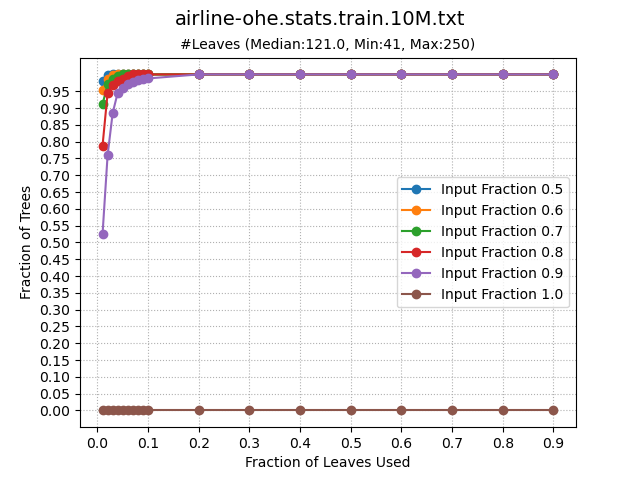
\includegraphics[width=\linewidth]{figures/airline-ohe.stats.train.txt.png}
    \caption{Statistical profile for airline-ohe}
    \label{Fig:AirlineOHEStats}
\end{figure}
\begin{figure}
    \centering
    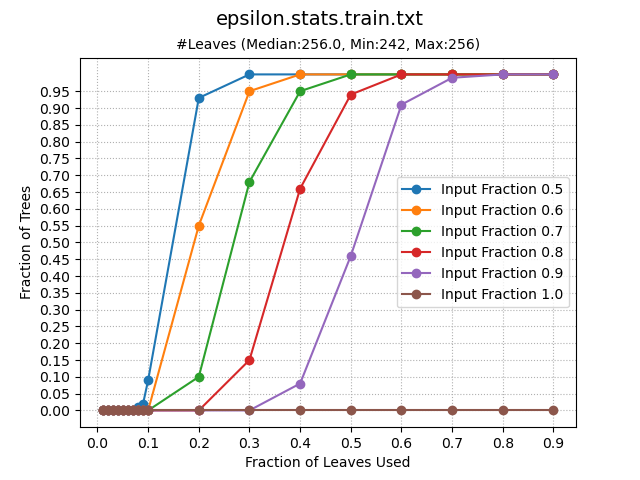
\includegraphics[width=\linewidth]{figures/epsilon.stats.train.txt.png}
    \caption{Statistical profile for epsilon}
    \label{Fig:EpsilonStats}
\end{figure}
\CommentOut{
We say that an input row $r_i$ is \textbf{\emph{covered}} by a subset of leaves $L' \subseteq L$ of a tree $T$, if the leaf $l$ reached by 
walking $T$ for row $r_i$ is in $L'$. We show how different models (and even different trees within the same model) behave differently 
using models for two benchmarks, airline-ohe and epsilon. Consider the graphs shown in   
figures \ref{Fig:AirlineOHEStats} and \ref{Fig:EpsilonStats}. Each line in these graphs corresponds to a fixed fraction of the input (say $f$). 
A point on a line at coordinate $(x, y)$ means that a fraction $y$ of trees in the model could cover a fraction $f$ of all training inputs with a fraction $x$ of 
leaves. For example, the first point on the $f=0.9$ line in figure \ref{Fig:AirlineOHEStats} says that about 52\% of trees ($y$ value) need only 1\% of their
leaves ($x$ value) to cover 90\% of the training input. 
In general, Figure \ref{Fig:AirlineOHEStats} shows that very few leaves are needed to cover a very large fraction of inputs for the benchmark airline-ohe. 
This means that a small fraction of leaves are very likely. On the other hand, for the benchmark epsilon,
figure \ref{Fig:EpsilonStats} shows that a trees need a much larger fraction of their leaves to cover a significant fraction of the test input.
This means that most trees in the epsilon model are not leaf biased.
One other observation we make is that most models have some leaf biased trees while the rest of the trees have equally likely leaves.
\TODO{AP Maybe define a term for trees with roughly equally likely leaves?} We design the probability based tiling algorithm to take advantage of this property 
of decision tree ensembles. 
}
\subsubsection{The Optimization Problem}

%We assume that we are given the probabilities of each leaf node of the decision tree (these can easily be computed using the training data). For every leaf $l \in L$, we %are given the probability $p_l$ that the leaf $l$ is reached. 

Observe that the latency of one tree walk is proportional to the number of tiles that need to be evaluated to reach the leaf. It is easy to see that for a leaf biased tree, basic tilling does not optimize for this objective, it considers all leafs to be equally likely. 
 
The goal of probablistic tiling is to minimize the average inference latency, or equivalently the minimize the expected number of tiles that are evaluated to compute one tree prediction. More formally, the problem is to find a \emph{valid} (as defined in Section~\ref{sec:ValidTiling}) tiling $\mathcal{T}$ such that the following objective is minimized.
\[
    \min_{\mathcal{T} \in \mathcal{C}(T)}{\sum_{l \in L_{\Tree}} p_l.depth_{\mathcal{T}}(l)}
\]
where the minimization is over all valid tilings $\mathcal{T}$ of the tree $\Tree$, $depth_{\mathcal{T}}(l)$ is the depth of the leaf $l$ given tiling ${\mathcal{T}}$. $p_l$ is the probability of of reaching leaf $l$ as observed during training.

The above optimization problem can be solved optimally using dynamic programming. 
We leave this out in the interest of space. 
Instead, we use the simple greedy algorithm listed in algorithm \ref{Alg:GreedyTilingAlgo} to construct a valid tiling given the node probabilities\footnote{Probabilites for internal nodes can be computed from probablities for leafs by summing up the probabilities of all leafs that belong to the sub-tree rooted at the internal node. Leaf probabilities are collected during training.}.
The algorithm starts at the root and greedily keeps adding the most probable legal node to the current tile until the maximum tile size is reached.
Subsequently, the tiling procedure is recursively performed on all nodes that are destinations for edges going out of the constructed tile.

% \subsubsection{Dynamic Programming Formulation}


% For any node $v \in V$, we define
% \[
%     cost(v, \mathcal{T}) = \sum_{l \in L_v} p(l | v).depth_{\mathcal{T}}(l)
% \]
% where $\mathcal{T} \in \mathcal{C}(T_v)$.

% Then, the objective function, for the tree $T_v$, can be rewritten as 
% \[
%     opt\_cost(v) = \min_{\mathcal{T} \in \mathcal{C}(T_v)}{cost(v, \mathcal{T})}
% \]

% The objective function can then be rewritten in the following recursive form.
% \[
%     opt\_cost(v) = \min_{T_0 \in TileShapes(n_t, v)}{1 + \sum_{(n_1, n_2) \in out(T_0)} p(n_1 | v)p(n_2 | n1)opt\_cost(n_2)}
% \]
% where $TileShapes(n_t, v)$ is the set of all tile shapes of size $n_t$ with root $v$. A straight forward substitution argument shows why the solution to the subproblems (tiling all sub-trees) needs to to be optimal. The objective is now in a form that can solved using
% dynamic programming. 

% \subsubsection{Greedy Algorithm}

% Intuitively, it seems like the following greedy algorithm also gives the optimal tiling. The algorithm starts at the root and greedily keeps adding the most probable node to the current tile until the maximum tile size is reached.
\begin{algorithm}
    \caption{Greedy Probability Based Tree Tiling}
    \label{Alg:GreedyTilingAlgo}
    \begin{algorithmic}
        \Procedure{TileTree}{$\Tree = (V, E, r)$, $n_t$} 
            \If {$r \in L_{\Tree}$}
                \State \textbf{return} $\{ r \}$
            \EndIf
            \State $Tile \leftarrow \{ r \}$
            \While{$|Tile| < n_t$}
                \State $e = (u,v) \in Out(Tile)$ st $p(v)$ is max and $v \notin L$
                \If{$e = \emptyset$}
                    \State \textbf{break}
                \EndIf
                \State $Tile = Tile \cup \{ v \}$
            \EndWhile
            \State $Tiles =  \{ Tile \}$
            \For{$(u,v) \in Out(Tile)$}
                \State $Tiles \leftarrow Tiles \cup TileTree(S_v, n_t)$
            \EndFor
            \State \textbf{return} $Tiles$
        \EndProcedure
    \end{algorithmic}
\end{algorithm}

% Talk about problems with increasing number of tile shapes and only performing such tiling on skewed trees
\CommentOut{
When we tried to apply algorithm \ref{Alg:GreedyTilingAlgo} on all trees in our benchmarks, we found
that even minor variations in probability caused the tiling algorithm to generate a large 
number of tile shapes. This in turn caused a loss in performance because the large size of the 
lookup table needed (section \ref{sec:LookupTable}) caused increased L1 cache misses. In order to 
alleviate this, we only perform probability based tiling on trees that are leaf biased.
}
We find probability based tiling is only beneficial for leaf biased trees\footnote{Turns out that for trees that are not leaf biased, probability based tiling produces many more tile shapes (see Section~\ref{sec:tileShapes}) which direclty impacts the cost of \op{getChildTile} making it more expensive than basic tiling.}.  Recall that   
a tree to be leaf biased if a small fraction of leaves, say $\alpha$, can cover a large fraction of training inputs, say $\beta$.
We only perform probability based tiling on trees with thresholds $\alpha=0.05$ and $\beta=0.9$ and fall back to uniform tiling otherwise. 





\subsection{A Note on Implementation}
\TODO{Kr : Not sure if this is needed}
The tiling algorithms generate a \op{TileId} attribute per tree. The \op{TileId} attribute contains a mapping from a Node to the TileId asigned to it.
This information is used when lowering to the mid level abstraction in the form of loops. A sample of the lowered MIR code is shown in Figure~\ref{Fig:Overview}.	